\documentclass[]{article}
\usepackage{polski}
\usepackage[utf8]{inputenc}
\usepackage{mathtools}
\usepackage{listings}
\usepackage{enumitem}
\usepackage{mathtools}
\usepackage{amsmath}
\usepackage{amssymb}
\usepackage{pgf,tikz}
\usepackage{mathrsfs}
\usepackage{graphicx}
\usetikzlibrary{arrows}
%opening
\let\normalint\int % PS
\def\int{\displaystyle\normalint} %PS
\title{\textbf{ Metody Numeryczne 2\\Laboratorium 6}\\
Metoda Rungego-Kutty rzędu trzeciego dla układu dwóch równań}
\author{Szymon Adach}

\begin{document}

\maketitle

\section{Treść zadania}
 \textbf{Zadanie 3:} Metoda Rungego-Kutty rzędu trzeciego ($r=3$) dla układu dwóch równań ($\alpha = 1$, $\beta = \frac{1}{2}$).
\section{Opis metody}
Rozwiązywany układ równań ma postać:
\begin{center}
	$\begin{cases} 
	y'(x) = f(x,y(x),z(x))\\
	z'(x) = g(x,y(x),z(x))
	\end{cases}$
\end{center}
Równanie to określone jest na przedziale $(a, b]$ dla warunkow początkowych $y_a=y(a)$, $z_a=z(a)$.
Ogólne wzory w metodzie Rungego-Kutty mają postać:
\begin{center}
	$y_{i+1}=y_i+h\cdot \sum\limits_{j=1}^{r}c_jk_j$\\
	$k_j=f(x_i+h\cdot \sum\limits_{l=1}^{j-1}b_{jl}, y_i + +h\cdot \sum_{l=1}^{j-1}b_{jl}k_l)$
\end{center}
Gdzie współczynniki $c_j$ oraz $b_{jl}$ spełniają:\\
\begin{center}
$\begin{bmatrix*}[r]
c_1 & 0 & 0\\
c_2 & b_{21} & 0\\
c_3 & b_{31} & b_{32}
\end{bmatrix*} = \begin{bmatrix*}[c]
1+\frac{2-3(\alpha+\beta)}{6\alpha\beta} & 0 & 0\\
\frac{3\beta-2}{6\alpha(\beta-\alpha)} & \alpha & 0\\
\frac{2-3\alpha}{6\beta(\beta-\alpha)} & \frac{3\alpha\beta(1-\alpha)-\beta^2}{\alpha(2-3\alpha)} & \frac{\beta(\beta-\alpha)}{\alpha(2-3\alpha)}\end{bmatrix*}
$
\newpage Dla $\alpha = 1$, $\beta = \frac{1}{2}$:
$\begin{bmatrix*}[r]
c_1 & 0 & 0\\
c_2 & b_{21} & 0\\
c_3 & b_{31} & b_{32}
\end{bmatrix*} = \begin{bmatrix*}[c]
\frac{1}{6} & 0 & 0\\
\frac{1}{6} &1 & 0\\
\frac{2}{3} & \frac{1}{4} & \frac{1}{4}
\end{bmatrix*} $
\end{center}
Modyfikacja metody dla układu dwóch równań da się zapisać jako:
	\begin{lstlisting}[mathescape, language=Matlab]
for m = 2:length(x)
k(1) = f(x(m-1), y(m-1), z(m-1));
l(1) = g(x(m-1), y(m-1), z(m-1));

k(2) = f(x(m-1) + h, y(m-1) + k(1) * h, z(m-1) + l(1) * h);
l(2) = g(x(m-1) + h, y(m-1) + k(1) * h, z(m-1) + l(1) * h); 

k(3) = f(x(m-1) + h/2, y(m-1) + h * ( 1/4 * k(1) + 1/4 * k(2)),...
z(m-1) + h * ( 1/4 * l(1) + 1/4 * l(2)));   
l(3) = g(x(m-1) + h/2, y(m-1) + h * ( 1/4 * k(1) + 1/4 * k(2)), ...
z(m-1) + h * ( 1/4 * l(1) + 1/4 * l(2)));

y(m) = y(m-1) + 1/6 * h * (k(1) + 4*k(2) + k(3));
z(m) = z(m-1) + 1/6 * h * (l(1) + 4*l(2) + l(3));
end	
	\end{lstlisting}
Współczynniki zostały podane jawnie - były wcześniej obliczone w celu przyspieszenia działania programu.
\section{Działanie programu}
Program jest uruchamiany poleceniem:
\begin{center}
	\textbf{RK3ODE(f, g, a, b, n, y\_a, z\_a)}
\end{center} 
\begin{itemize}
	\item \textbf{f} - uchwyt do funkcji f(x,y,z)
	\item \textbf{g} - uchwyt do funkcji g(x,y,z)
	\item \textbf{a,b} - poczatek i koniec przedziału
	\item \textbf{n} - liczba węzłów
	\item \textbf{y\_a} - warunek początkowy $y(a) = y_a$
	\item \textbf{z\_a} - warunek początkowy $z(a) = z_a$
\end{itemize}
Funkcja ta zwraca wektory $y$, $z$ zawierające obliczone wartości $y_i$, $z_i$ dla węzłów. Jednak w celu graficznej prezentacji wyników należy uruchomić:
\begin{center}
	\textbf{test\_rk3ode(s, n)}
	\begin{itemize}
		\item \textbf{s} - numer przykładu (liczba od 1 do 3)
		\item \textbf{n} - liczba węzłów
	\end{itemize}
\end{center} 
Po uruchomieniu w dolnej i górnej części ekranu prezentowane są wykresy rozwiązań jednego z trzech przykładowych układów równań. W każdym oknie rysowane są wykresy rozwiązania dokładnego oraz znalezionego metodą Rungego-Kutty. Ponadto w konsoli wypisywany jest komunikat:\\
\verb|Max blad y(x) = |\\
\verb|Max blad z(x) = |
\section{Przykłady}
\begin{enumerate}
\item \textbf{Wywołanie:}\\
$y'=z$,\hspace{16mm}      $y(0)=1$\\
$z'=-2y-z$,\hspace{5mm}    $z(0)=1$\\
$(a,b] = (0,10]$
\\
\verb|test_rk3ode(1, 500)|
\\\textbf{Wyjście:}\\
\verb|Max blad y(x)=0.003230|\\
\verb|Max blad z(x)=0.006594|\\
\textbf{Rozwiązanie dokładne:} $y(x)= e^{-x}(2x+1)$, \\$z(x)= e^{-x}(1-2x)$
\begin{center}
	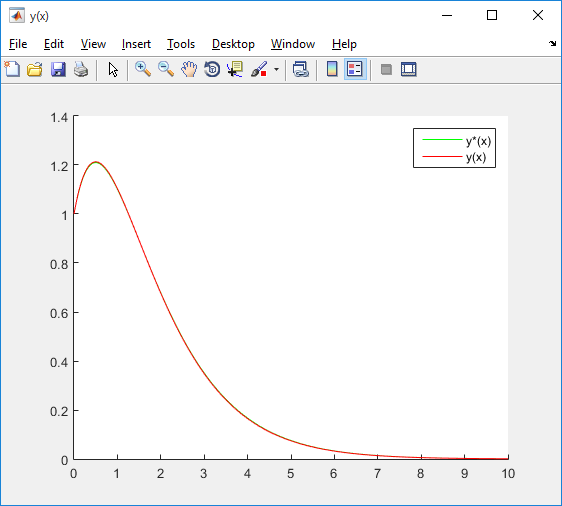
\includegraphics[scale=0.7]{y1.png}\\
	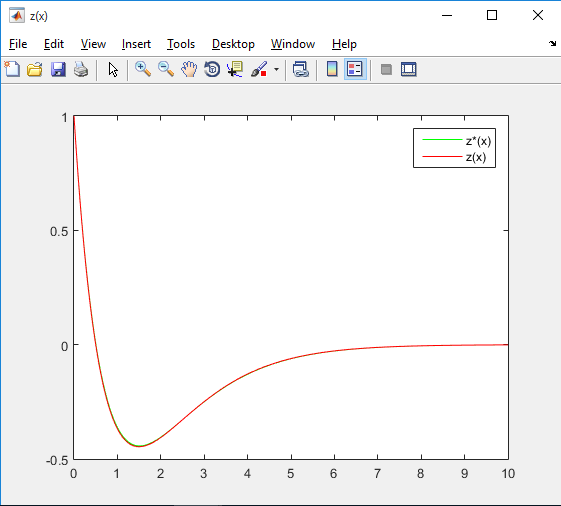
\includegraphics[scale=0.85]{z1.png}
\end{center}

\item \textbf{Wywołanie:}\\
$y'=y+5z$,\hspace{8mm}      $y(0)=2$\\
$z'=-y-3z$,\hspace{5mm}   $z(0)=1$\\
$(a,b] = (0,10]$
\\
\verb|test_rk3ode(2, 100)|
\\\textbf{Wyjście:}\\
\verb|Max blad y(x)=0.139011|\\
\verb|Max blad z(x)=0.079480|\\
\textbf{Rozwiązanie dokładne:}\\ $y(x)= e^{-x}(9\sin (x)+2\cos (x)$,\\ $z(x)= e^{-x}(\cos(x)-4sin(x))$
\begin{center}
	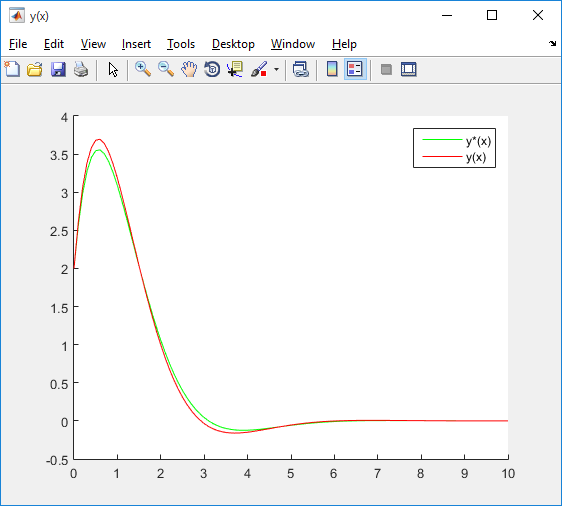
\includegraphics[scale=0.7]{y2.png}\\
	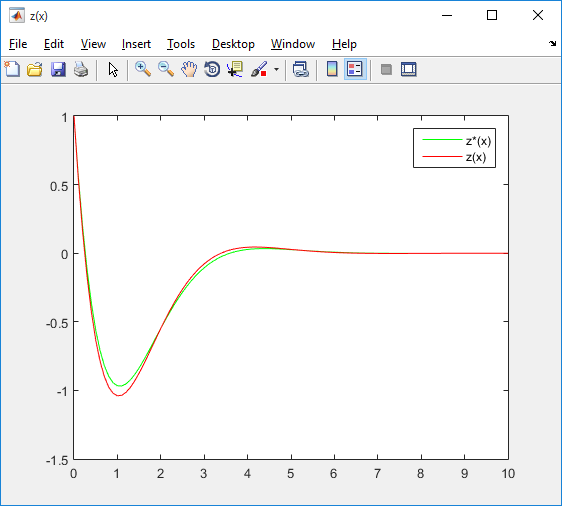
\includegraphics[scale=0.7]{z2.png}
\end{center}
\item \textbf{Wywołanie:}\\
$y'=2y$,\hspace{7mm}      $y(1)=2e^2$\\
$z'=yz^2$,\hspace{5mm}   $z(1)=\frac{1}{2-e^{2}}$\\
$(a,b] = (1,11]$
\\
\verb|test_rk3ode(3, 1000)|
\\\textbf{Wyjście:}\\
\verb|Max blad y(x)=730545494.058938|\\
\verb|Max blad z(x)=0.000343|\\
\textbf{Rozwiązanie dokładne:}\\ $y(x)= 2e^{2x}$,\\ $z(x)= \frac{1}{2-e^{2x}}$
\begin{center}
	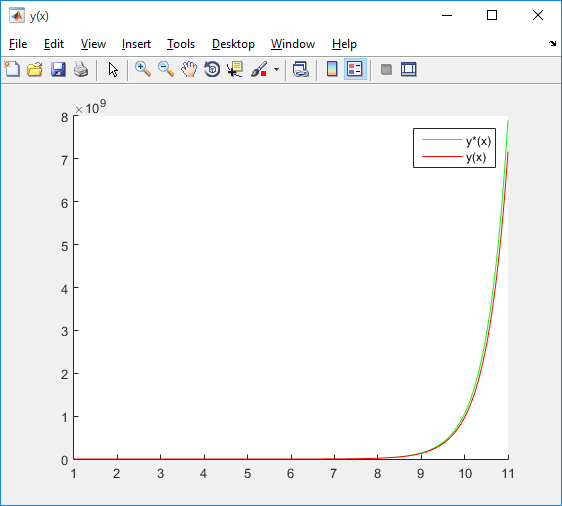
\includegraphics[scale=0.8]{y3.png}\\
	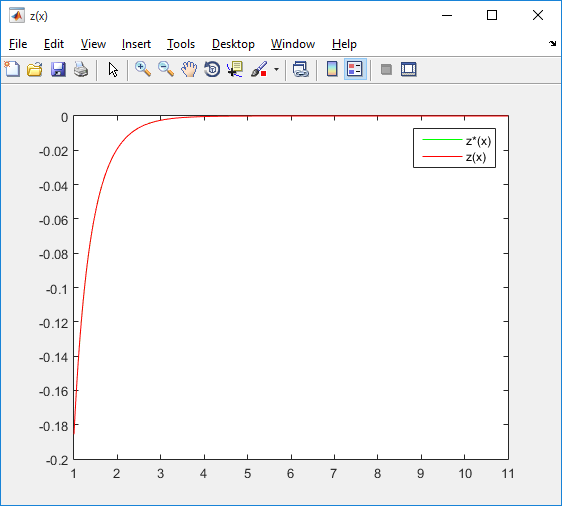
\includegraphics[scale=0.8]{z3.png}
\end{center}
\end{enumerate}
\end{document}
